%!TEX root = main.tex 
\documentclass{beamer}

\usepackage[utf8]{inputenc}
\usepackage[T1]{fontenc}
\usepackage[english,brazil]{babel}
\usepackage{booktabs}
\usepackage{tabularx}
\usepackage{graphicx}

% usando tema personalizado. 
% arquivo beamerthemeIFSC.sty deve estar no mesmo diretório do .tex
\usepackage{beamerthemeIFSC}

\usepackage[font=tiny]{caption} 

\title{Sistemas de Transmissão CVT}
\subtitle{Fundamentos, Evolução e o Sistema Direct Shift}
\author{Lucas Cechin Mário \and André Ghisleni Raimann}
\institute{Instituto Federal de Santa Catarina — Campus Chapecó}
\date{2026}

\begin{document}

  \begin{frame}
  \titlepage
  \end{frame}

  \section{Introdução}

  \begin{frame}{Conceito e Motivação}
      \begin{block}{O que é o CVT?}
      A Transmissão Continuamente Variável (CVT) não possui um número limitado de engrenagens com relações fixas, permitindo transição ininterrupta.
      \end{block}
      
      \begin{itemize}
          \item \textbf{Eficiência:} Mantém o motor sempre em sua faixa de potência ideal.
          \item \textbf{Demanda de Mercado:} Busca global por redução de emissões e menor consumo de combustível.
          \item \textbf{Conforto:} Elimina os solavancos ("trancadas") típicos de trocas de marcha convencionais.
      \end{itemize}
  \end{frame}

  \section{Contexto Histórico}

  \begin{frame}{Evolução Tecnológica}
      \begin{itemize}
          \item \textbf{Séc. XV:} Conceito idealizado por Leonardo da Vinci.
          \item \textbf{1886:} Primeira patente por Daimler e Benz.
          \item \textbf{Anos 1950:} Sistema \textit{Variomatic} introduzido pela DAF (Holanda). O primeiro a ser aplicado em automóveis de produção.
          \item \textbf{Atualidade:} Amplo domínio japonês (Toyota, Nissan, Honda, Subaru) em veículos de passeio.
      \end{itemize}
      
      \vspace{0.3cm}
      % Descomente abaixo após colocar a imagem na pasta
      % \begin{center}
      %   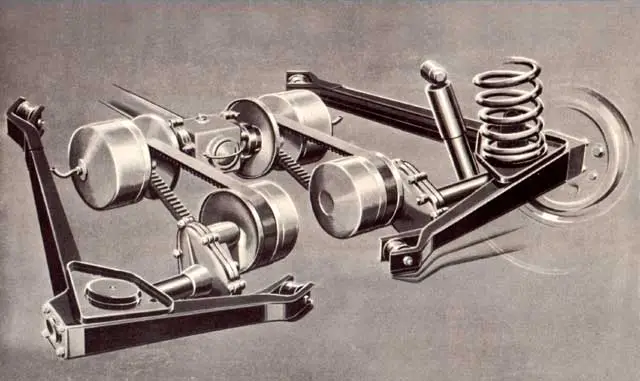
\includegraphics[width=0.4\textwidth]{images/daf_variomatic.jpg}
      %   \captionof{figure}{\tiny Sistema DAF Variomatic antigo.}
      % \end{center}
  \end{frame}

  \section{Fundamentos Mecânicos}

  \begin{frame}{Polias e Correia}
    \begin{columns}
      \column{0.55\textwidth}
      O sistema clássico baseia-se em geometria variável:
      \begin{enumerate}
          \item \textbf{Polia Primária:} Motriz (ligada ao motor).
          \item \textbf{Polia Secundária:} Movida (ligada às rodas).
          \item \textbf{Dinâmica:} O afastamento/aproximação das faces cônicas altera o diâmetro efetivo da correia metálica.
          \item \textbf{Ponto Morto:} Na marcha lenta, a correia gira no menor diâmetro possível da polia primária.
      \end{enumerate}

      \column{0.45\textwidth}
      % \centering
      % 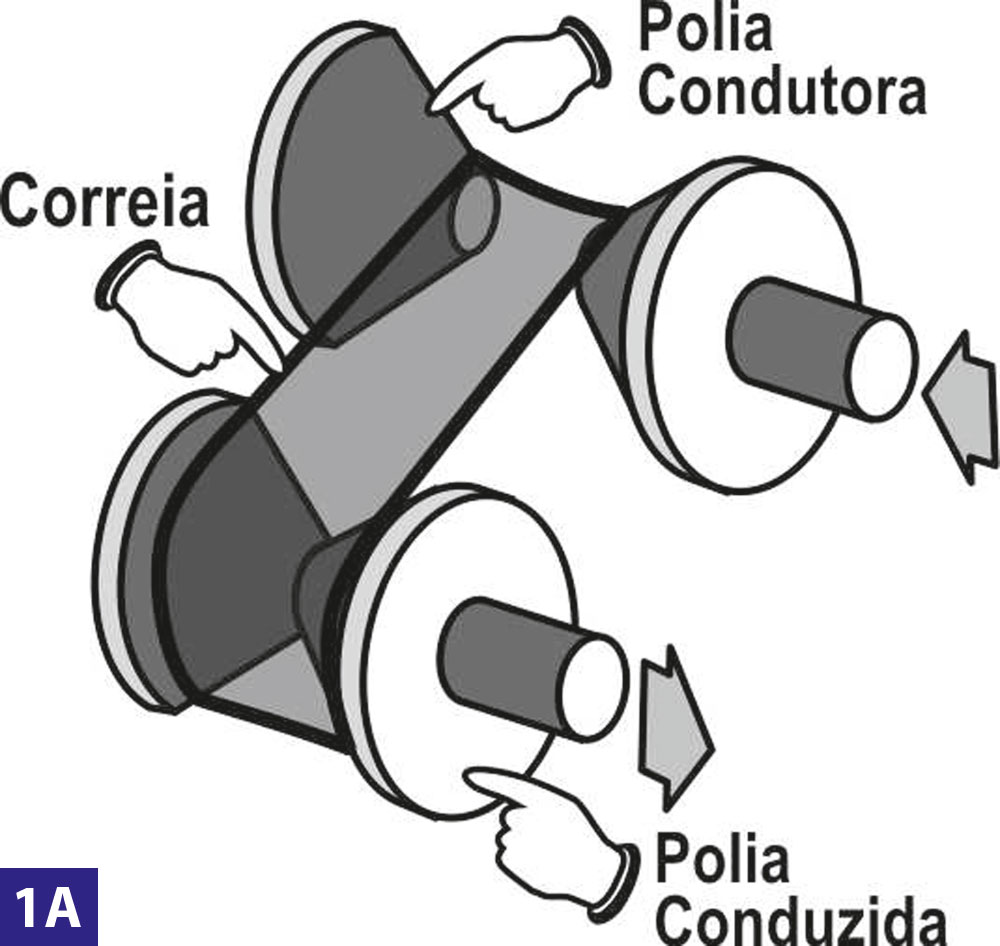
\includegraphics[width=0.9\textwidth]{images/polias_cvt.png}
      % \captionof{figure}{\tiny Conjunto de polias cônicas.}
    \end{columns}
  \end{frame}

  \section{Inovação: Direct Shift-CVT}

  \begin{frame}{Visão Aprimorada: Direct Shift-CVT}
      \begin{block}{O Problema do CVT Clássico}
      Baixa eficiência em relações iniciais, causando sensação de lentidão na arrancada e desgaste prematuro das polias.
      \end{block}
      
      \textbf{A Solução da Toyota (ex: K120):}
      \begin{itemize}
          \item Incorpora uma \textbf{engrenagem física de arrancada} (\textit{launch gear}).
          \item O carro arranca pelo sistema de engrenagens e, ao ganhar velocidade, a transição para as polias ocorre suavemente.
          \item \textbf{Benefício Mecânico:} Inércia das polias reduzida em 40\%, agilizando trocas e melhorando consumo em até 6\%.
      \end{itemize}
  \end{frame}

  \section{Manutenção e Diagnóstico}

  \begin{frame}{Sistemas de Controle}
      A operação mecânica depende de uma malha eletro-hidráulica precisa:
      \begin{itemize}
          \item \textbf{Pressão de Linha:} Avaliação requer manômetros de até 1.000 psi conectados nas portas de verificação (ex: transmissões JATCO).
          \item \textbf{Controles vitais:} Atuação do LockUp (conversor de torque) e pressões aplicadas nas polias.
          \item \textbf{Desgaste:} Óleo fora da especificação ou rolamentos fadigados geram limalha severa no cárter, comprometendo o corpo de válvulas e causando trepidações.
      \end{itemize}
  \end{frame}

  \section{Análise de Viabilidade}

  \begin{frame}{Vantagens vs. Desafios}
    \begin{columns}[T]
        \begin{column}{0.5\textwidth}
            \textbf{Vantagens}
            \begin{itemize}
                \item Alta eficiência térmica e rendimento de combustível (até 16 km/l em sedãs).
                \item Suavidade extrema (ausência de solavancos).
                \item Aceleração linear e responsiva.
                \item Menos peças móveis que um automático de engrenagens.
            \end{itemize}
        \end{column}
        
        \begin{column}{0.5\textwidth}
            \textbf{Desafios e Desvantagens}
            \begin{itemize}
                \item \textit{Drone Noise}: Motor estático em alta rotação passa sensação de "patinar".
                \item Limitação de Torque, dificultando uso em trabalho pesado/esportivos.
                \item Durabilidade da correia e altíssimo custo de substituição estrutural.
            \end{itemize}
        \end{column}
    \end{columns}
  \end{frame}

  \section{Conclusão}

  \begin{frame}{Considerações Finais}
    \begin{block}{Revitalização da Engenharia Clássica}
    O câmbio CVT exemplifica como hardwares mecânicos tradicionais podem ser reinventados através de lógicas de controle de alta fidelidade.
    \end{block}
    
    \vspace{0.5cm}
    A adoção de esquemas híbridos, mesclando engrenagens de arraste com polias de baixa inércia, prova que ainda existe vasta margem para a otimização de trens de força, solucionando falhas antigas de confiabilidade.
  \end{frame}

  \section{Referências}

    \begin{frame}{Referências Técnicas}
    \begin{block}{Literatura e Fontes Consultadas}
        \begin{itemize}
            \item BUDYNAS, R. G.; NISBETT, J. K. \textbf{Shigley's Mechanical Engineering Design}. 11th Edition. McGraw-Hill Education, 2019.
            \item TOYOTA MOTOR CORPORATION / AISIN. \textbf{Toyota Direct Shift-CVT (K120) Technical Documentation}. Press Release e Plataformas Automotivas, 2018.
            \item JATCO LTD. \textbf{CVT Service and Diagnostic Manuals: Avaliação e Controle Eletro-hidráulico}. Manuais técnicos de bancada e manutenção.
            \item BOSCH TRANSMISSION TECHNOLOGY. \textbf{Histórico e catálogos técnicos de desenvolvimento de correias push-belt (Van Doorne/Variomatic)}.
            \item SINDIREPA MT. \textbf{Reparação de transmissões CVT: diagnósticos, testes de pressão e falhas comuns}. 2021.
        \end{itemize}
    \end{block}
    \end{frame}

  \begin{frame}
    \centering
    \vspace{1cm}
    \Large \textbf{Obrigado!} \\
    \vspace{0.5cm}
    \normalsize Lucas Cechin Mário e André Ghisleni Raimann \\
    Engenharia de Controle e Automação — IFSC
  \end{frame}

\end{document}